
\chapter{METODOLOGI PENELITIAN}
\label{cha:3-MetodologiPenelitian}

\section{Gambaran Umum} \label{sec:3-GambaranUmum}

Penelitian ini membahas pemanfaatan data gambar sebagai acuan dalam melakukan pelatihan dan
implementasi model \textit{deep neural network} untuk mencari dan memetakan koordinat tiga dimensi
pose tubuh manusia dalam sebuah rangkaian gambar secara lokal. Pengerjaan aplikasi mengutamakan dua
langkah penting yang meliputi pengolahan data dan pembuatan model. Aplikasi yang dibuat dapat menampilkan
plot grafik tiga dimensi menyerupai struktur anatomi tubuh manusia sesuai dengan pose hasil
estimasi dari gambar masukkan. Hasil pelatihan model ditampilkan dalam grafik dua dimensi untuk
analisis lebih lanjut.

\textit{Dataset} yang digunakan dalam penelitian ini terbagi menjadi dua jenis yang meliputi
\textit{dataset} pembuatan model dan \textit{dataset} inferensi aplikasi.
\textit{Dataset} pembuatan model dikategorikan menjadi data pelatihan model dan data validasi model.
\textit{Dataset} pembuatan model berisi gambar dan target posisi titik kunci anatomi dalam jumlah besar.
Data pelatihan model adalah data yang digunakan dalam proses pelatihan sebagai sampel bagi \textit{deep neural network}.
Data validasi model adalah data yang digunakan untuk menguji kebenaran fungsionalitas pemetaan yang
dipelajari saat pelatihan model. \textit{Dataset} inferensi aplikasi adalah data uji coba berbentuk
video tanpa target titik kunci yang digunakan untuk estimasi pose tubuh manusia secara sekuensial.

Pelatihan model \textit{deep neural network} diimplementasikan menggunakan \textit{framework} PyTorch.
Kedua \textit{dataset} yang digunakan diolah terlebih dahulu sehingga memenuhi syarat PyTorch dalam melakukan
\textit{deep learning}.
Setiap model kemudian digunakan terhadap \textit{dataset} inferensi
aplikasi. Proses dan hasil estimasi diurai lebih lanjut dalam bentuk grafik visual.

\section{Kerangka Penelitian} \label{sec:3-KerangkaPenelitian}

Kerangka penelitian yang jelas dibutuhkan untuk memudahkan proses penelitian sehingga dapat
mempersingkat waktu pengerjaan. Proses penelitian dibagi menjadi tiga tahapan besar yang meliputi
tahap praproduksi, tahap produksi, dan tahap uji coba. Setiap tahapan tersebut dikerjakan secara
terurut dan sistematis. Alur setiap tahap diilustrasikan pada gambar~\ref{fig:kerangkapenelitian}.

\begin{figure}[htbp]
    \begin{center}
        \fbox{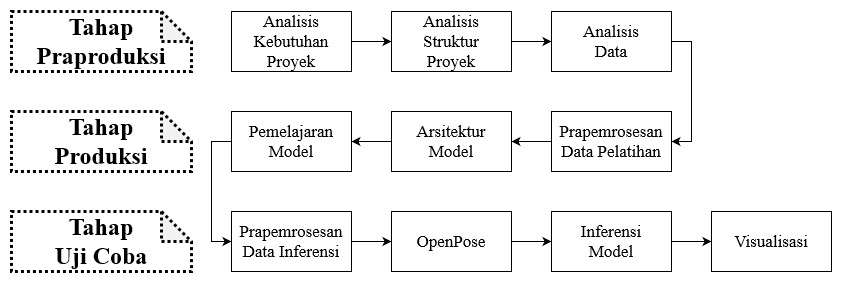
\includegraphics[width=11.9cm]{bab3/gambar/kerangka_penelitian.jpg}}
    \end{center}
    \vspace{-20pt}
    \captionsetup{labelfont=bf, textfont=bf}
    \caption{Kerangka Penelitian}
    \vspace{-10pt}
    \captionsetup{labelfont=md, textfont=md}
    % \caption*{Sumber: sumber}
    % \caption*{Sumber: nama(2019)}
    \label{fig:kerangkapenelitian}
\end{figure}

\section{Tahap Praproduksi} \label{sec:3-TahapPraproduksi}

Tahap praproduksi berisi langkah-langkah analisis yang menentukan alur pada tahap selanjutnya. Tahap
praproduksi dibagi menjadi beberapa langkah yang meliputi analisis kebutuhan proyek, analisis
struktur proyek, dan analisis data. Tahap ini menganalisis bagian-bagian pokok yang diperlukan
sehingga mengetahui langkah-langkah yang akan dilakukan pada tahap produksi.

\subsection{Analisis Kebutuhan Proyek}

Pelatihan dan implementasi model ini memerlukan alat-alat pendukung berupa perangkat keras dan
perangkat lunak yang mencukupi. Spesifikasi perangkat keras dan perangkat lunak yang lebih besar
akan mempercepat proses pelatihan model jaringan saraf tiruan.
Spesifikasi perangkat keras yang digunakan dalam penelitian ini
dapat dilihat pada tabel~\ref{tab:spesifikasiperangkatkeras}. Spesifikasi perangkat lunak yang
digunakan dalam penelitian ini dapat dilihat pada tabel~\ref{tab:spesifikasiperangkatlunak}.


\begin{table}[htbp]
    \captionsetup{labelfont=bf, textfont=bf}
    \caption{Spesifikasi Perangkat Keras}
    \label{tab:spesifikasiperangkatkeras}
    \vspace{-20pt}
    \begin{center}
        \begin{tabular}{|c|c|}
            \hline
            \multicolumn{2}{|c|}{\textbf{Perangkat Keras (Laptop)}} \\ \hline
            CPU & Intel Core I7 7700 HQ                             \\ \hline
            GPU & NVIDIA GTX 1060 6 GB                              \\ \hline
            RAM & 24 GB DDR4                                        \\ \hline
            SSD & NVME SAMSUNG 120 GB                               \\ \hline
            HDD & SATA 1 TB                                         \\ \hline
            % \multicolumn{1}{|c|}{RDF-3X}    & a & b & c & d & e & f & g \\ \hline
        \end{tabular}
    \end{center}
\end{table}

\begin{table}[htbp]
    \captionsetup{labelfont=bf, textfont=bf}
    \caption{Spesifikasi Perangkat Lunak}
    \label{tab:spesifikasiperangkatlunak}
    \vspace{-20pt}
    \begin{center}
        \begin{tabular}{|c|c|}
            \hline
            \multicolumn{2}{|c|}{\textbf{Perangkat Lunak}} \\ \hline
            Sistem Operasi      & Ubuntu 19.10             \\ \hline
            IDE                 & Jupyter Lab              \\ \hline
            Bahasa Pemrograman  & Python 3.7               \\ \hline
            \textit{Framework } & PyTorch 1.4              \\ \hline
        \end{tabular}
    \end{center}
\end{table}

\subsection{Analisis Struktur Proyek}

Perancangan struktur proyek yang sistematis diperlukan untuk meminimalisir kompleksitas dalam
melakukan pembuatan dan pelatihan model. \textit{Integrated development environment} Jupyter Lab
memudahkan eksekusi perintah dengan sintaks bahasa pemrograman Python dalam bentuk sel interaktif.
Setiap sel terdiri dari
\textit{input} dan \textit{output}. Sel \textit{input} berisi perintah yang akan dieksekusi, sedangkan
sel \textit{output} berisi hasil eksekusi yang dapat berupa teks ataupun grafik. Cara kerja Jupyter Lab
dapat dilihat pada gambar~\ref{fig:jupyterlab}.
\begin{figure}[htbp]

    \begin{center}
        \fbox{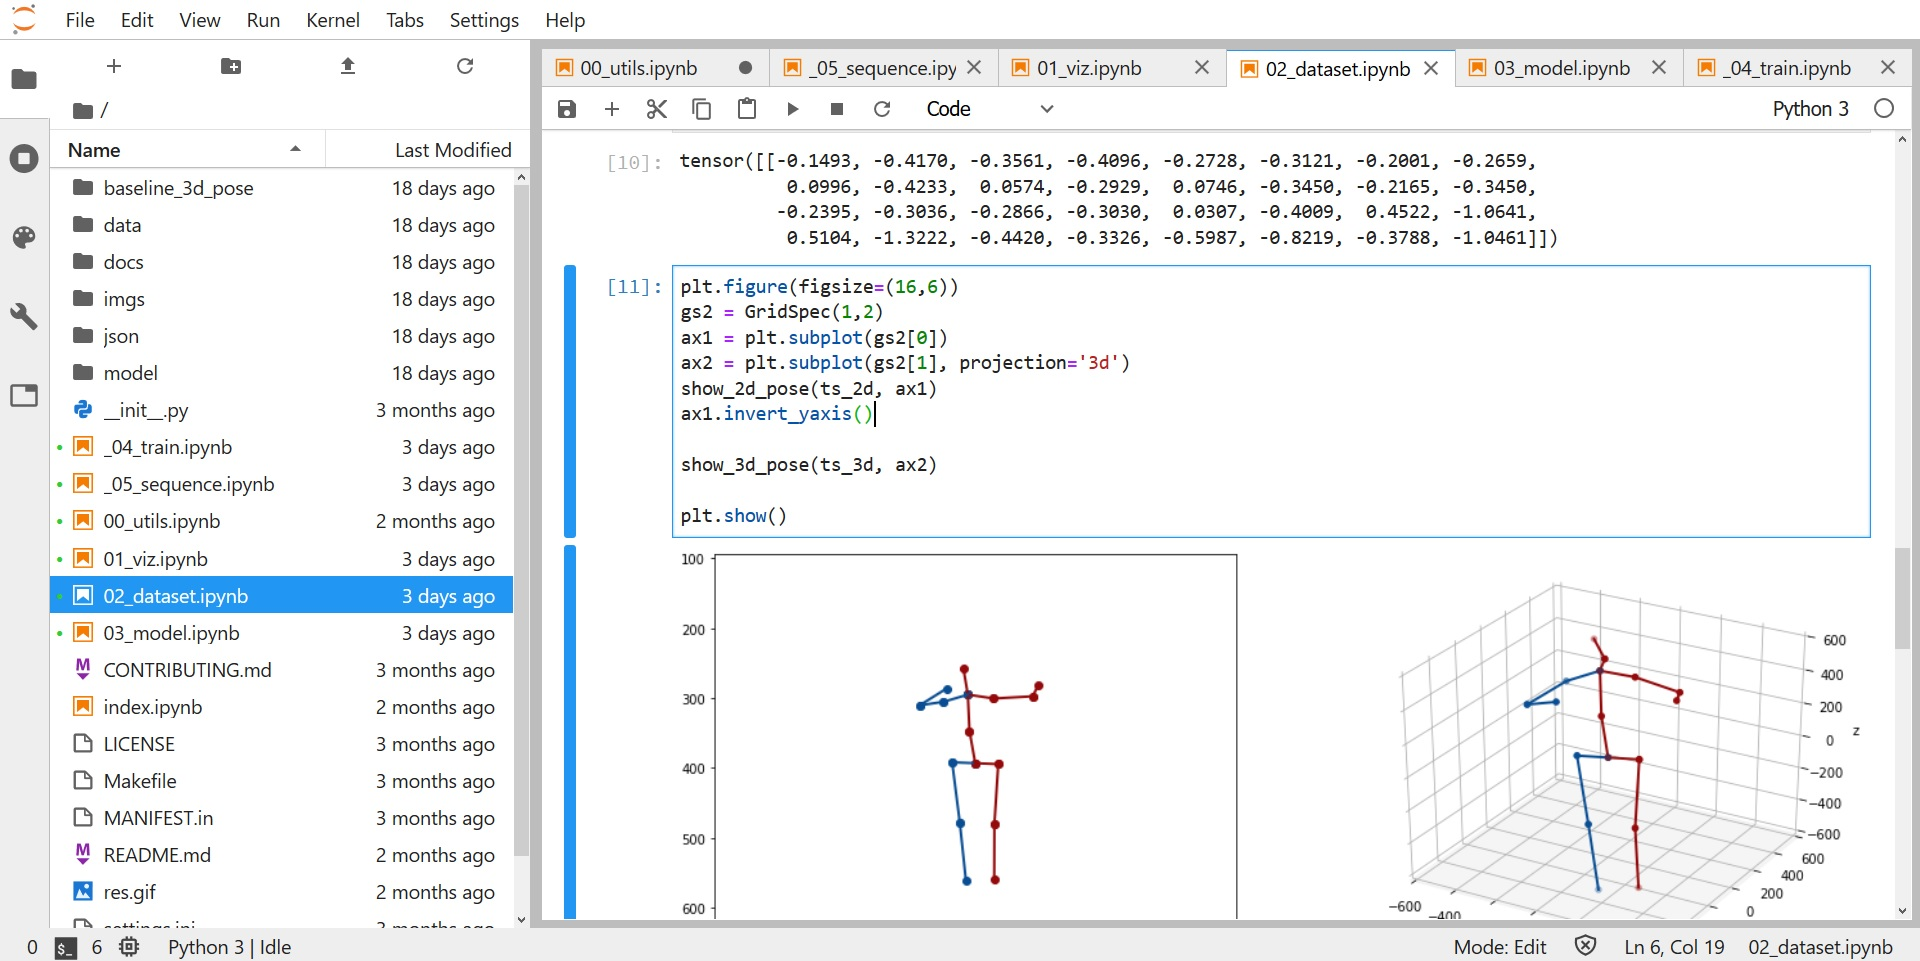
\includegraphics[width=11.9cm]{bab3/gambar/jupyterlab.jpg}}
    \end{center}
    \vspace{-20pt}
    \captionsetup{labelfont=bf, textfont=bf}
    \caption{Jupyter Lab}
    \vspace{-10pt}
    \captionsetup{labelfont=md, textfont=md}
    % \caption*{Sumber: sumber}
    % \caption*{Sumber: nama(2019)}
    \label{fig:jupyterlab}
\end{figure}

\subsection{Analisis Data}
Data Latihan
Data Inferensi

\section{Tahap Produksi} \label{sec:3-TahapProduksi}

\subsection{Prapemrosesan Data Pelatihan}
Kelas DataLoader

\subsection{Arsitektur Model}
DNN

\subsection{Pelatihan Model}


\section{Tahap Uji Coba} \label{sec:3-TahapUjiCoba}

\subsection{Prapemrosesan Data Inferensi}

\subsection{OpenPose}

\subsection{Inferensi Model}

\subsection{Visualisasi}

\begin{table}[htbp]
    \captionsetup{labelfont=bf, textfont=bf}
    \caption{Sebuah tabel}
    \vspace{-20pt}
    \begin{center}
        \begin{tabular}{| l c r |}
            \hline
            1 & 2 & 3 \\
            4 & 5 & 6 \\
            7 & 8 & 9 \\
            \hline
        \end{tabular}
    \end{center}
    \vspace{-10pt}
    \captionsetup{labelfont=md, textfont=md}
    % \caption*{Sumber: Bego Lu}
\end{table}